\section{Implementación del Diseño}

\subsection{Descripción del Sistema}
El objetivo del diseño es la automatización de un montacargas de tres niveles. El sistema debe ser capaz de recibir comandos de llamada desde tres pulsadores ($P1, P2, P3$), detectar la posición de la cabina mediante finales de carrera ($fc1, fc2, fc3$) y controlar tanto el motor de tracción como un indicador visual de posición.

El núcleo del control se basa en una \textbf{Máquina de Estados Finitos (FSM)} que gestiona la lógica secuencial del movimiento. Debido a la necesidad de una respuesta inmediata de las salidas (indicadores de motor y display) ante cambios en las entradas, se optó por una arquitectura de \textbf{Máquina de Mealy}.

\subsection{Máquina de Estados Finita (FSM)}
La FSM diseñada consta de 7 estados lógicos, codificados en un registro de 3 bits. La selección del modelo de Mealy permite que las salidas ($S$ para el motor y $D$ para el display) dependan tanto del estado actual como de las entradas presentes, lo que reduce la latencia en la indicación de las acciones.



\tikzset{every picture/.style={line width=0.75pt}} %set default line width to 0.75pt

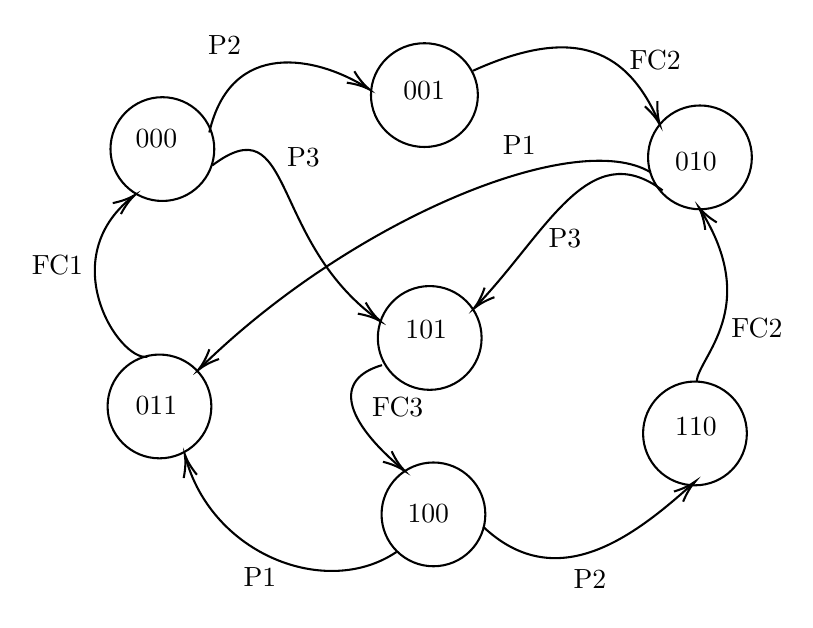
\begin{tikzpicture}[x=0.75pt,y=0.75pt,yscale=-1,xscale=1]
%uncomment if require: \path (0,432); %set diagram left start at 0, and has height of 432

%Shape: Circle [id:dp8422975507173965]
\draw   (107,71) .. controls (107,57.19) and (118.19,46) .. (132,46) .. controls (145.81,46) and (157,57.19) .. (157,71) .. controls (157,84.81) and (145.81,96) .. (132,96) .. controls (118.19,96) and (107,84.81) .. (107,71) -- cycle ;
%Flowchart: Connector [id:dp7678102365376042]
\draw   (232.5,45) .. controls (232.5,31.19) and (244.03,20) .. (258.25,20) .. controls (272.47,20) and (284,31.19) .. (284,45) .. controls (284,58.81) and (272.47,70) .. (258.25,70) .. controls (244.03,70) and (232.5,58.81) .. (232.5,45) -- cycle ;
%Shape: Circle [id:dp9236195072271722]
\draw   (366,75) .. controls (366,61.19) and (377.19,50) .. (391,50) .. controls (404.81,50) and (416,61.19) .. (416,75) .. controls (416,88.81) and (404.81,100) .. (391,100) .. controls (377.19,100) and (366,88.81) .. (366,75) -- cycle ;
%Shape: Circle [id:dp20177079502880357]
\draw   (237.6,247) .. controls (237.6,233.19) and (248.79,222) .. (262.6,222) .. controls (276.41,222) and (287.6,233.19) .. (287.6,247) .. controls (287.6,260.81) and (276.41,272) .. (262.6,272) .. controls (248.79,272) and (237.6,260.81) .. (237.6,247) -- cycle ;
%Shape: Circle [id:dp8972357128166435]
\draw   (105.6,195) .. controls (105.6,181.19) and (116.79,170) .. (130.6,170) .. controls (144.41,170) and (155.6,181.19) .. (155.6,195) .. controls (155.6,208.81) and (144.41,220) .. (130.6,220) .. controls (116.79,220) and (105.6,208.81) .. (105.6,195) -- cycle ;
%Shape: Circle [id:dp5547460354385172]
\draw   (363.6,208) .. controls (363.6,194.19) and (374.79,183) .. (388.6,183) .. controls (402.41,183) and (413.6,194.19) .. (413.6,208) .. controls (413.6,221.81) and (402.41,233) .. (388.6,233) .. controls (374.79,233) and (363.6,221.81) .. (363.6,208) -- cycle ;
%Curve Lines [id:da5115956921605481]
\draw    (154.6,63) .. controls (164.99,17.63) and (206.49,26.32) .. (230.36,41.37) ;
\draw [shift={(231.8,42.3)}, rotate = 213.47] [color={rgb, 255:red, 0; green, 0; blue, 0 }  ][line width=0.75]    (10.93,-3.29) .. controls (6.95,-1.4) and (3.31,-0.3) .. (0,0) .. controls (3.31,0.3) and (6.95,1.4) .. (10.93,3.29)   ;
%Curve Lines [id:da7788845060307221]
\draw    (281.7,33.25) .. controls (326.52,13.01) and (354.36,19.5) .. (370.95,57.49) ;
\draw [shift={(371.7,59.25)}, rotate = 247.35] [color={rgb, 255:red, 0; green, 0; blue, 0 }  ][line width=0.75]    (10.93,-3.29) .. controls (6.95,-1.4) and (3.31,-0.3) .. (0,0) .. controls (3.31,0.3) and (6.95,1.4) .. (10.93,3.29)   ;
%Curve Lines [id:da9753865787641531]
\draw    (367.3,82.25) .. controls (331.48,60.36) and (223.49,104.55) .. (150.3,176.41) ;
\draw [shift={(149.2,177.5)}, rotate = 315.28] [color={rgb, 255:red, 0; green, 0; blue, 0 }  ][line width=0.75]    (10.93,-3.29) .. controls (6.95,-1.4) and (3.31,-0.3) .. (0,0) .. controls (3.31,0.3) and (6.95,1.4) .. (10.93,3.29)   ;
%Curve Lines [id:da7786642901677974]
\draw    (156,78.9) .. controls (195.6,49.2) and (183.25,114.57) .. (235.4,152.75) ;
\draw [shift={(237,153.9)}, rotate = 215.13] [color={rgb, 255:red, 0; green, 0; blue, 0 }  ][line width=0.75]    (10.93,-3.29) .. controls (6.95,-1.4) and (3.31,-0.3) .. (0,0) .. controls (3.31,0.3) and (6.95,1.4) .. (10.93,3.29)   ;
%Shape: Circle [id:dp3878777355879428]
\draw   (235.8,162) .. controls (235.8,148.19) and (246.99,137) .. (260.8,137) .. controls (274.61,137) and (285.8,148.19) .. (285.8,162) .. controls (285.8,175.81) and (274.61,187) .. (260.8,187) .. controls (246.99,187) and (235.8,175.81) .. (235.8,162) -- cycle ;
%Curve Lines [id:da8587692145450346]
\draw    (373,90.9) .. controls (337.36,64.17) and (317.4,110.95) .. (283.05,146.82) ;
\draw [shift={(282,147.9)}, rotate = 314.19] [color={rgb, 255:red, 0; green, 0; blue, 0 }  ][line width=0.75]    (10.93,-3.29) .. controls (6.95,-1.4) and (3.31,-0.3) .. (0,0) .. controls (3.31,0.3) and (6.95,1.4) .. (10.93,3.29)   ;
%Curve Lines [id:da9730101438239867]
\draw    (389.4,182.95) .. controls (390.29,171.12) and (420.78,147.43) .. (391.31,100.38) ;
\draw [shift={(390.4,98.95)}, rotate = 57.14] [color={rgb, 255:red, 0; green, 0; blue, 0 }  ][line width=0.75]    (10.93,-3.29) .. controls (6.95,-1.4) and (3.31,-0.3) .. (0,0) .. controls (3.31,0.3) and (6.95,1.4) .. (10.93,3.29)   ;
%Curve Lines [id:da841036905553302]
\draw    (237.8,175.1) .. controls (214.16,182) and (219.63,201.5) .. (247.51,225.02) ;
\draw [shift={(248.8,226.1)}, rotate = 219.61] [color={rgb, 255:red, 0; green, 0; blue, 0 }  ][line width=0.75]    (10.93,-3.29) .. controls (6.95,-1.4) and (3.31,-0.3) .. (0,0) .. controls (3.31,0.3) and (6.95,1.4) .. (10.93,3.29)   ;
%Curve Lines [id:da4451319303070028]
\draw    (286.6,253) .. controls (322.26,286.59) and (359.85,257.11) .. (387.54,232.23) ;
\draw [shift={(388.8,231.1)}, rotate = 137.92] [color={rgb, 255:red, 0; green, 0; blue, 0 }  ][line width=0.75]    (10.93,-3.29) .. controls (6.95,-1.4) and (3.31,-0.3) .. (0,0) .. controls (3.31,0.3) and (6.95,1.4) .. (10.93,3.29)   ;
%Curve Lines [id:da8282928641033299]
\draw    (244.8,265.1) .. controls (211.14,287.87) and (155.92,266.54) .. (143.17,219.53) ;
\draw [shift={(142.8,218.1)}, rotate = 75.96] [color={rgb, 255:red, 0; green, 0; blue, 0 }  ][line width=0.75]    (10.93,-3.29) .. controls (6.95,-1.4) and (3.31,-0.3) .. (0,0) .. controls (3.31,0.3) and (6.95,1.4) .. (10.93,3.29)   ;
%Curve Lines [id:da5885541061829214]
\draw    (124.8,171.1) .. controls (111.14,173.18) and (79.44,124.1) .. (117.62,94.01) ;
\draw [shift={(118.8,93.1)}, rotate = 143.13] [color={rgb, 255:red, 0; green, 0; blue, 0 }  ][line width=0.75]    (10.93,-3.29) .. controls (6.95,-1.4) and (3.31,-0.3) .. (0,0) .. controls (3.31,0.3) and (6.95,1.4) .. (10.93,3.29)   ;

% Text Node
\draw (117.6,60) node [anchor=north west][inner sep=0.75pt]  [font=\normalsize] [align=left] {000};
% Text Node
\draw (246.6,37) node [anchor=north west][inner sep=0.75pt]  [font=\normalsize] [align=left] {001};
% Text Node
\draw (377.6,71) node [anchor=north west][inner sep=0.75pt]   [align=left] {010};
% Text Node
\draw (377.6,199) node [anchor=north west][inner sep=0.75pt]   [align=left] {110};
% Text Node
\draw (247.6,152) node [anchor=north west][inner sep=0.75pt]   [align=left] {101};
% Text Node
\draw (248.6,241) node [anchor=north west][inner sep=0.75pt]   [align=left] {100};
% Text Node
\draw (117.6,189) node [anchor=north west][inner sep=0.75pt]   [align=left] {011};
% Text Node
\draw (67.6,121) node [anchor=north west][inner sep=0.75pt]   [align=left] {FC1};
% Text Node
\draw (152.6,15) node [anchor=north west][inner sep=0.75pt]   [align=left] {P2};
% Text Node
\draw (355.6,22) node [anchor=north west][inner sep=0.75pt]   [align=left] {FC2};
% Text Node
\draw (190.6,69) node [anchor=north west][inner sep=0.75pt]   [align=left] {P3};
% Text Node
\draw (294.6,63) node [anchor=north west][inner sep=0.75pt]   [align=left] {P1};
% Text Node
\draw (316.6,108) node [anchor=north west][inner sep=0.75pt]   [align=left] {P3};
% Text Node
\draw (231.6,189) node [anchor=north west][inner sep=0.75pt]   [align=left] {FC3};
% Text Node
\draw (169.6,271) node [anchor=north west][inner sep=0.75pt]   [align=left] {P1};
% Text Node
\draw (328.6,272) node [anchor=north west][inner sep=0.75pt]   [align=left] {P2};
% Text Node
\draw (404.6,151) node [anchor=north west][inner sep=0.75pt]   [align=left] {FC2};


\end{tikzpicture}


\subsubsection{Definición de Estados}
Los estados se clasifican en dos categorías funcionales:
\begin{itemize}
    \item \textbf{Estados de Reposo (Estacionarios):} Representan la permanencia del montacargas en un piso específico.
    \begin{itemize}
        \item \textbf{PISO 1:} Estado inicial y de reposo en el primer nivel. Salidas: $S=00$ (Quieto), $D=1$ (Piso 1).
        \item \textbf{PISO 2:} Estado de reposo en el segundo nivel. Salidas: $S=00$, $D=2$.
        \item \textbf{PISO 3:} Estado de reposo en el tercer nivel. Salidas: $S=00$, $D=3$.
    \end{itemize}
    \item \textbf{Estados de Transición (Movimiento):} Representan el desplazamiento de la cabina entre niveles.
    \begin{itemize}
        \item \textbf{SUBE 2:} Movimiento ascendente hacia el piso 2. Salidas: $S=01$ (Sube), $D=$ Apagado.
        \item \textbf{SUBE 3:} Movimiento ascendente hacia el piso 3. Salidas: $S=01$, $D=$ Apagado.
        \item \textbf{BAJA 1:} Movimiento descendente hacia el piso 1. Salidas: $S=10$ (Baja), $D=$ Apagado.
        \item \textbf{BAJA 2:} Movimiento descendente hacia el piso 2. Salidas: $S=10$, $D=$ Apagado.
    \end{itemize}
\end{itemize}

\subsubsection{Lógica de Transiciones}
El diagrama de estados se comporta de la siguiente manera:
\begin{enumerate}
    \item Estando en \textbf{PISO 1}: Si se activa $P2$, transita a \textit{SUBE 2}. Si se activa $P3$, transita a \textit{SUBE 3}.
    \item Estando en \textbf{SUBE 2}: Permanece en este estado hasta que $fc2$ se activa, momento en el que transita a \textit{PISO 2}.
    \item Estando en \textbf{PISO 2}: Si se activa $P3$, transita a \textit{SUBE 3}. Si se activa $P1$, transita a \textit{BAJA 1}.
    \item Estando en \textbf{SUBE 3}: Permanece en este estado hasta que $fc3$ se activa, provocando la transición a \textit{PISO 3}.
    \item Estando en \textbf{PISO 3}: Si se activa $P2$, transita a \textit{BAJA 2}. Si se activa $P1$, transita a \textit{BAJA 1}.
    \item Estando en \textbf{BAJA 2} o \textbf{BAJA 1}: El sistema mantiene el movimiento descendente hasta que se activa el final de carrera correspondiente ($fc2$ o $fc1$), retornando al estado de reposo respectivo.
\end{enumerate}

\subsection{Salidas del Sistema}
El comportamiento de las salidas en función del estado y las entradas se resume a continuación:
\begin{itemize}
    \item \textbf{Motor (S):} 2 bits. '00' detiene el motor, '01' activa la subida y '10' activa la bajada.
    \item \textbf{Display (D):} 7 bits. Muestra el número del piso actual solo cuando el montacargas está detenido (en estados PISO X). Durante los estados de movimiento, el display permanece apagado para indicar tránsito.
\end{itemize}
